\subsubsection{誤差逆伝搬法の近似による教師あり学習}

ANNは誤差逆伝搬法(Back-propagation)を用いてパラメータを学習することができますが、SNNは誤差逆伝搬法を直接使用することはできません。しかし、誤差逆伝搬法の近似をすることでSNNを訓練することができるようになります。SNNを誤差逆伝搬法で訓練することは\textbf{SpikeProp法}(Bohte et al., 2000)や\textbf{ReSuMe}(Ponulak, Kasiński, 2010)など多数の手法が考案されてきました(他の方針としては Lee et al. 2016\footnote{この論文のポイントは実数値の膜電位で確率的勾配降下を実行することです。}; Huh \& Sejnowski, 2018; Wu et al., 2018; Shrestha \& Orchard, 2018; Tavanaei \& Maida, 2019; Thiele et al., 2019; Comsa et al., 2019など多数)。この章の初めでは、代表してSpikeProp法の改善手法であ\textbf{るSuperSpike法}(Zenke and Ganguli, 2018)の実装をしてみます。
\section{SuperSpike法}
\textbf{SuperSpike法} (supervised learning rule for spiking neurons)(Zenke and Ganguli, 2018)はオンラインの教師あり学習でSpikeProp法と同様にスパイク列を教師信号とし、そのスパイク列を出力するようにネットワークを最適化します。SpikeProp法と異なるのはスパイクの微分ではなく、膜電位についての関数の微分を用いていることです。このため、発火が生じなくても学習が進行します。
\subsection{損失関数の導関数の近似}
まず最小化したい損失関数$L$から考えましょう。$i$番目のニューロンの教師信号となるスパイク列$\hat{S}_{i}$に出力${S}_{i}$を近づけます(スパイク列は$S_i(t)=\sum_{t_{k}< t} \delta\left(t-t_i^{k}\right)$と表されます)\footnote{通常、予測値に$\hat{}$を付けることが多いですが、ここでは論文の表記に従って$\hat{S}$を教師信号としています。}。SpikeProp法ではこれらの二乗誤差を損失関数としていましたが、SuperSpike法ではそれぞれのスパイク列を二重指数関数フィルター$\alpha$で畳み込みした後に二乗誤差を取ります。
\begin{equation}
L(t)=\frac{1}{2} \int_{-\infty}^{t} d s\left[\left(\alpha * \hat{S}_{i}-\alpha * S_{i}\right)(s)\right]^{2}
\end{equation}
ただし、$*$は畳み込み演算子です。これは\textbf{van Rossum 距離} (van Rossum, 2001)\footnote{スパイク列の類似度を計算する手法としては他にVictor-Purpura 距離や、 Schreiber \textit{et al.}類似度など、数多く考案されています。(Dauwels et al., 2008)やScholarpediaの"Measures of spike train synchrony"(\url{http://www.scholarpedia.org/article/Measures_of_spike_train_synchrony})を参照してください。}を表します。損失関数をこのように設定することで、SpikePropと異なり、完全にスパイク列が一致するまで誤差信号は0になりません。
損失関数$L$を$j$番目のシナプス前ニューロンから$i$番目のシナプス後ニューロンへのシナプス強度$w_{ij}$で微分すると、次のようになります。
\begin{equation}
\frac{\partial L}{\partial w_{i j}}=-\int_{-\infty}^{t} d s\left[\left(\alpha * \hat{S}_{i}-\alpha * S_{i}\right)(s)\right]\left(\alpha * \frac{\partial S_{i}}{\partial w_{i j}}\right)(s)    
\end{equation}
目標はこの$\dfrac{\partial L}{\partial w_{i j}}$を計算し、確率的勾配降下法(stochastic gradient discent; SGD)により$w_{ij}\leftarrow w_{ij}-r \dfrac{\partial L}{\partial w_{i j}}$と最適化することです(ただし$r$は学習率)。ここでの問題点は$\dfrac{\partial S_{i}}{\partial w_{i j}}$の部分です。$S_i$は$\delta$関数を含むため、微分すると発火時は$\infty$, 非発火時は0となり、学習が進みません。そこで$S_i(t)$をLIFニューロンの膜電位\footnote{これまで$V$や$v$を使っていましたが、論文にあわせて$U$を用います。}$U_i(t)$の非線形関数$\sigma(U_i(t))$で近似します。非線形関数としては高速シグモイド関数(fast sigmoid) $\sigma(x)=x/(1+|x|)$を使用しています。ここまでの近似計算を纏めると
\begin{equation}
\frac{\partial S_{i}}{\partial w_{ij}}\approx\frac{\partial \sigma\left(U_{i}\right)}{\partial w_{ij}}=\sigma^{\prime}\left(U_{i}\right) \frac{\partial U_{i}}{\partial w_{i j}}    
\end{equation}
となります。ただし、$\sigma^{\prime}\left(U_{i}\right)=(1+|\beta(U_i-\vartheta)|)^{-2}$です。$\vartheta$はLIFニューロンの発火閾値で$-$50 mVとされています。$\beta$は係数で(1 mV)$^{-1}$です。\par
残った$\dfrac{\partial U_{i}}{\partial w_{i j}}$の部分ですが、シナプス強度$w_{ij}$の変化により$j$番目のシナプス前ニューロンの発火$S_j(t)$が$i$番目のシナプス後細胞の膜電位変化に与える影響が変化するという観点から、$\dfrac{\partial U_{i}}{\partial w_{i j}}\approx \epsilon* S_j(t)$と近似します。ただし、$\epsilon$は$\alpha$と同じ二重指数関数フィルターです。また、これはシナプスでの神経伝達物質の濃度として解釈できるとされています。\par
ここまでの近似を用いると、時刻$t$におけるシナプス強度の変化率$\dfrac{\partial w_{ij}}{\partial t}$は
\begin{align}
\frac{\partial w_{ij}}{\partial t}&=-r \dfrac{\partial L}{\partial w_{i j}}\\
&\approx r\int_{-\infty}^{t} ds\underbrace{\left[\alpha * \left(\hat{S}_{i}-S_{i}\right)(s)\right]}_{誤差信号}\quad\alpha *\left[ \underbrace{\sigma^{\prime}\left(U_{i}(s)\right)}_{後細胞}\underbrace{\left(\epsilon * S_{j}\right)(s)}_{前細胞}\right]\\
&=r\int_{-\infty}^{t} ds\ \ e_i(s)\cdot \lambda_{ij}(s)
\end{align}
と表せます。ここで、$e_i(t)=\alpha * \left(\hat{S}_{i}-S_{i}\right)$, $\lambda_{ij}(t)=\alpha *\left[\sigma^{\prime}\left(U_{i}(s)\right)\left(\epsilon * S_{j}\right)(s)\right]$としました。$e_i(t)$は誤差信号(error signal)で、シナプス前細胞にフィードバックされます。$\lambda_{ij}(t)$はシナプス適格度トレース(synaptic eligibility trace)を表します\footnote{これは遅延報酬問題(distal reward problem)を解決していると説明されています。また、生理学的にはCa$^{2+}$トランジェント(calcium transient)や関連するシグナル伝達カスケード(signaling cascade)として実現可能であるとされています。}。\par
\subsection{離散化した重みの更新とRMaxProp}
前項における$\dfrac{\partial w_{ij}}{\partial t}$ は時刻$t$までの全ての誤差情報を積分していますが、実装する上での利便性を考え、時刻$[t_k, t_{k+1}]$ の間の積分を用いて重みを更新します\footnote{これはミニバッチによる更新に類似しています。}。
\begin{equation}
\Delta w_{i j}^{k}=r_{ij} \int_{t_{k}}^{t_{k+1}} e_{i}(s) \lambda_{ij}(s) ds      
\end{equation}
ただし、$r_{ij}$は重み$w_{ij}$ごとの学習率です(これは後で説明します)。さらに実装時には$t_b:={t_{k+1}}-{t_{k}}\ (=0.5$ s)とし、0で初期化されている配列[$m_{ij}$]をステップごとに
\begin{equation}
m_{ij} \leftarrow m_{ij} + g_{ij}    
\end{equation}
という式により更新します。ただし、$g_{ij}=e_{i}(t) \lambda_{ij}(t)$です。$t_b$だけ経過すると、
\begin{equation}
w_{ij} \leftarrow w_{ij} + r_{ij}m_{ij}\cdot \Delta t
\end{equation}
として重み$w_{ij}$を更新し、$m_{ij}$を0にリセットします\footnote{$\Delta t$は元の論文には記載されていないですが、タイムステップの長さが変化しても良いようにするためにつけています。}。さらに更新時は重みに$-1<w_{ij}<1$という制限をつけています。\par
学習率$r$は全ての重みに対して同じものを用いても学習は可能ですが、安定はしません。そこで、ANNのOptimizerの一種である\textbf{RMSprop}と類似した更新を行います。\par
まず、新しく配列$[v_{ij}]$を用意します。タイムステップごとに
v_{ij} \leftarrow \max(\gamma v_{ij}, g_{ij}^2)
で更新します。ただし、$\gamma$はハイパーパラメータです(明確な値の記載がありませんが、実験の結果から0.8程度の値がよいでしょう)。この$v_{ij}$を用いて重みごとの学習率$r_{ij}$を次のように定義します。
\begin{equation}
r_{ij}=\frac{r_0}{\sqrt{v_{ij}}+\varepsilon}
\end{equation}
ただし、$r_0$は学習係数、$\varepsilon$はゼロ除算を避けるための小さい値(典型的には$\varepsilon=10^{-8}$)です。記載はありませんが、学習係数の減衰(learning rate decay)を行うと学習がよく進みました。\par
以上の更新法を著者らは\textbf{RMaxProp}と名付けています。なお、RMSpropの場合は$g_{ij}^2$の移動平均を次式のように行います。
v_{ij} \leftarrow \gamma v_{ij}+(1-\gamma)\cdot g_{ij}^2
\subsection{誤差信号の逆伝搬について}
出力層において誤差信号は$e_i(t)=\alpha * \left(\hat{S}_{i}-S_{i}\right)$と計算されます。これを低次の層に逆伝搬すること、つまり$l$層目の$k$番目のニューロンの誤差信号$e_k$を$l-1$層目の$i$番目のニューロンに投射することを考えます。対称なフィードバックをする場合、$W=[w_{ik}]$の転置行列$W^\intercal=[w_{ki}]$を用いて、
\begin{equation}
e_i=\sum_k w_{ki} e_k
\end{equation}
となります。ここでANNの誤差逆伝搬のように、$l-1$番目の層の出力を引数とする活性化関数の勾配を乗じません。\par
この対称フィードバックは順伝搬の重みの転置行列を用いるため、生物学的には妥当ではありません。そこで誤差逆伝搬法の対称な重みを使う問題を解消する手法として\textbf{Feedback alignment} (Lillicrap et al., 2016)があります\footnote{Feedback alignmentの発展については(Nøkland 2016; Akrout et al., 2019; Lansdell et al 2019)を参照してください。}。Feedback alignmentでは逆伝搬時に用いる重みをランダムに固定したものとします\footnote{なぜこれが上手くいくかを書く時間がありませんでした。論文を読んでください。}。このとき、ランダムな固定重みを$B=[b_{ki}]$とすると、Feedback alignmentの場合は
\begin{equation}
e_i=\sum_k b_{ki} e_k
\end{equation}
となります。また、重みを均一なものとするUniform feedbackによる学習も紹介されています。この場合は、
\begin{equation}
e_i=\sum_k e_k
\end{equation}
となります。後の実装ではFeedback alignmentによる学習も行います。

\subsection{SuperSpike法の実装}
それではSuperSpike法を実装していきましょう。今回は3層のネットワーク(ユニット数は順に50, 4, 1)の出力ユニットが100 msごとに発火するように訓練します。 訓練後の結果と全体のアルゴリズムは図\ref{fig:super_spike}にまとめていますので、適宜参照すると良いでしょう。。\par
まず、\texttt{Models}ディレクトリの親ディレクトリに実行するファイルを作成します。次に今回使うモデルをimportしておきます。
\begin{minted}[frame=lines, framesep=2mm, baselinestretch=1.2, bgcolor=shadecolor,fontsize=\small]{python}
from Models.Neurons import CurrentBasedLIF
from Models.Synapses import DoubleExponentialSynapse
from Models.Connections import FullConnection, DelayConnection
\end{minted}
\subsubsection{誤差信号と適格度トレースの実装}
まず、誤差信号と適格度トレースの計算を行うclassを実装します。とはいえ、二重指数関数型シナプスのコードに少し変更を加えるだけでよいです。異なる点として、誤差信号では出力層のスパイク列(\texttt{output\_spike})と教師信号のスパイク列(\texttt{target\_spike})を引数とし、それらの差分を取ります。さらにこの時、出力が$[-1, 1]$となるように規格化を行います。
\begin{minted}[frame=lines, framesep=2mm, baselinestretch=1.2, bgcolor=shadecolor,fontsize=\small]{python}
class ErrorSignal:
    def __init__(self, N, dt=1e-4, td=1e-2, tr=5e-3):
        self.dt = dt
        self.td = td
        self.tr = tr
        self.N = N
        self.r = np.zeros(N)
        self.hr = np.zeros(N)
        self.b = (td/tr)**(td/(tr-td)) \section{規格化定数}
    
    def initialize_states(self):
        self.r = np.zeros(self.N)
        self.hr = np.zeros(self.N)    

    def __call__(self, output_spike, target_spike):
        r = self.r*(1-self.dt/self.tr) + self.hr/self.td*self.dt 
        hr = self.hr*(1-self.dt/self.td)+(target_spike-output_spike)/self.b
        self.r = r
        self.hr = hr
        return r
\end{minted}
次に、適格度トレースはシナプス前細胞のシナプスフィルターをかけられたスパイク列と、シナプス後細胞の膜電位を引数とします。シナプス後細胞の膜電位は高速シグモイド関数の微分した式に代入され、Online STDP\footnote{5章参照}の計算のように列ベクトル(postの活動)と行ベクトル(preの活動)の積を取ります。
\begin{minted}[frame=lines, framesep=2mm, baselinestretch=1.2, bgcolor=shadecolor,fontsize=\small]{python}
lass EligibilityTrace:
    def __init__(self, N_in, N_out, dt=1e-4, td=1e-2, tr=5e-3):
        self.dt = dt
        self.td = td
        self.tr = tr
        self.N_in = N_in
        self.N_out = N_out
        self.r = np.zeros((N_out, N_in))
        self.hr = np.zeros((N_out, N_in))
    
    def initialize_states(self):
        self.r = np.zeros((self.N_out, self.N_in))
        self.hr = np.zeros((self.N_out, self.N_in))
    
    def surrogate_derivative_fastsigmoid(self, u, beta=1, vthr=-50):
        return 1 / (1 + np.abs(beta*(u-vthr)))**2

    def __call__(self, pre_current, post_voltage):
        \section{(N_out, 1) x (1, N_in) -> (N_out, N_in) }
        pre_ = np.expand_dims(pre_current, axis=0)
        post_ = np.expand_dims(
                self.surrogate_derivative_fastsigmoid(post_voltage), 
                axis=1)
        r = self.r*(1-self.dt/self.tr) + self.hr*self.dt 
        hr = self.hr*(1-self.dt/self.td) + (post_ @ pre_)/(self.tr*self.td)
        self.r = r
        self.hr = hr
        return r
\end{minted}
\subsubsection{定数とモデルの定義}
それでは準備が終わったので、定数とモデルのインスタンスを定義しましょう。
\begin{minted}[frame=lines, framesep=2mm, baselinestretch=1.2, bgcolor=shadecolor,fontsize=\small]{python}
dt = 1e-4; T = 0.5; nt = round(T/dt)

t_weight_update = 0.5 #重みの更新時間
nt_b = round(t_weight_update/dt) #重みの更新ステップ

num_iter = 200 \section{学習のイテレーション数}

N_in = 50 \section{入力ユニット数}
N_mid = 4 \section{中間ユニット数}
N_out = 1 \section{出力ユニット数}

\section{入力(x)と教師信号(y)の定義}
fr_in = 10 \section{入力のPoisson発火率 (Hz)}
x = np.where(np.random.rand(nt, N_in) < fr_in * dt, 1, 0)
y = np.zeros((nt, N_out)) 
y[int(nt/10)::int(nt/5), :] = 1 \section{T/5に1回発火}

\section{モデルの定義}
neurons_1 = CurrentBasedLIF(N_mid, dt=dt)
neurons_2 = CurrentBasedLIF(N_out, dt=dt)
delay_conn1 = DelayConnection(N_in, delay=8e-4)
delay_conn2 = DelayConnection(N_mid, delay=8e-4)
synapses_1 = DoubleExponentialSynapse(N_in, dt=dt, td=1e-2, tr=5e-3)
synapses_2 = DoubleExponentialSynapse(N_mid, dt=dt, td=1e-2, tr=5e-3)
es = ErrorSignal(N_out)
et1 = EligibilityTrace(N_in, N_mid)
et2 = EligibilityTrace(N_mid, N_out)

connect_1 = FullConnection(N_in, N_mid, 
                           initW=0.1*np.random.rand(N_mid, N_in))
connect_2 = FullConnection(N_mid, N_out, 
                           initW=0.1*np.random.rand(N_out, N_mid))
#B = np.random.rand(N_mid, N_out) \section{Feedback alignment}

r0 = 1e-3
gamma = 0.7

\section{記録用配列}
current_arr = np.zeros((N_mid, nt))
voltage_arr = np.zeros((N_out, nt))
error_arr = np.zeros((N_out, nt))
lambda_arr = np.zeros((N_out, N_mid, nt))
dw_arr = np.zeros((N_out, N_mid, nt))
cost_arr = np.zeros(num_iter)
\end{minted}
ここで配列\texttt{B}はFeedback alignmentの際に用います。
\subsubsection{シミュレーションの実装}
\texttt{for}ループ内でモデルを構築し、\texttt{nt\_b}ステップごとに重みの更新を行います。また、最後の訓練イテレーション時に、出力層の膜電位の時間変化などを記録しておきます。
\begin{minted}[frame=lines, framesep=2mm, baselinestretch=1.2, bgcolor=shadecolor,fontsize=\small]{python}
for i in tqdm(range(num_iter)):
    if i%15 == 0:
        r0 /= 2 \section{重み減衰}
    
    \section{状態の初期化}
    neurons_1.initialize_states()
    neurons_2.initialize_states()
    synapses_1.initialize_states()
    synapses_2.initialize_states()
    delay_conn1.initialize_states()
    delay_conn2.initialize_states()
    es.initialize_states()
    et1.initialize_states()
    et2.initialize_states()
    
    m1 = np.zeros((N_mid, N_in))
    m2 = np.zeros((N_out, N_mid))
    v1 = np.zeros((N_mid, N_in))
    v2 = np.zeros((N_out, N_mid))
    cost = 0
    count = 0
    
    \section{one iter.}
    for t in range(nt):
        \section{Feed-forward}
        c1 = synapses_1(delay_conn1(x[t])) \section{input current}
        h1 = connect_1(c1)
        s1 = neurons_1(h1) \section{spike of mid neurons}
        
        c2 = synapses_2(delay_conn2(s1))
        h2 = connect_2(c2)
        s2 = neurons_2(h2)
        
        \section{Backward(誤差の伝搬)}
        e2 = np.expand_dims(es(s2, y[t]), axis=1) / N_out
        e1 = connect_2.backward(e2) / N_mid
        \section{e1 = np.dot(B, e2) / N_mid}

        \section{コストの計算}
        cost += np.sum(e2**2)
        
        lambda2 = et2(c2, neurons_2.v_)
        lambda1 = et1(c1, neurons_1.v_)
        
        g2 = e2 * lambda2
        g1 = e1 * lambda1
        
        v1 = np.maximum(gamma*v1, g1**2)
        v2 = np.maximum(gamma*v2, g2**2)
        
        m1 += g1
        m2 += g2
    
        count += 1
        if count == nt_b:
            \section{重みの更新}
            lr1 = r0/np.sqrt(v1+1e-8)
            lr2 = r0/np.sqrt(v2+1e-8)
            dW1 = np.clip(lr1*m1*dt, -1e-3, 1e-3)
            dW2 = np.clip(lr2*m2*dt, -1e-3, 1e-3)
            connect_1.W = np.clip(connect_1.W+dW1, -0.1, 0.1)
            connect_2.W = np.clip(connect_2.W+dW2, -0.1, 0.1)
            
            \section{リセット}
            m1 = np.zeros((N_mid, N_in))
            m2 = np.zeros((N_out, N_mid))
            v1 = np.zeros((N_mid, N_in))
            v2 = np.zeros((N_out, N_mid))
            count = 0
            
        \section{保存}
        if i == num_iter-1:
            current_arr[:, t] = c2
            voltage_arr[:, t] = neurons_2.v_
            error_arr[:, t] = e2
            lambda_arr[:, :, t] = lambda2
    
    cost_arr[i] = cost
    print("\n cost:", cost)
\end{minted}
なお、\texttt{r}は重みの係数ですが、これを減衰させる(つまりweight decay)するとパフォーマンスが上がったので、今回冒頭に入れています。また、\texttt{lr}は更新時の値を用いていますが、これはANNにおいて入力ごとの勾配を加算し、重みの更新はミニバッチ内の全ての要素に対して同じ学習率で行うということに対応します。また、Feedback alignmentの場合は誤差逆伝搬に\colorbox{shadecolor}{\texttt{e1 = np.dot(B, e2) / N\_mid}}を用います。
\subsubsection{結果の描画}
最後に結果を描画します。描画するのは出力層の膜電位$U_i$, 高速シグモイドによる膜電位の微分の近似$\sigma^\prime (U_i)$, 出力層における誤差信号$e_i$, 適格度トレース$\lambda_{ij}$, 2層目の$j=0$番目のシナプス後電流$\epsilon * S_j$, 入力のポアソンスパイク、誤差関数の推移です。
\begin{minted}[frame=lines, framesep=2mm, baselinestretch=1.2, bgcolor=shadecolor,fontsize=\small]{python}
t = np.arange(nt)*dt*1e3

plt.figure(figsize=(8, 10))
plt.subplot(6,1,1)
plt.plot(t, voltage_arr[0])
plt.ylabel('Membrane\n potential (mV)')
plt.subplot(6,1,2)
plt.plot(t, et1.surrogate_derivative_fastsigmoid(u=voltage_arr[0]))
plt.ylabel('Surrogate derivative')
plt.subplot(6,1,3)
plt.plot(t, error_arr[0])
plt.ylabel('Error')
plt.subplot(6,1,4)
plt.plot(t, lambda_arr[0, 0], color="k")
plt.ylabel('$\lambda$')
plt.subplot(6,1,5)
plt.plot(t, current_arr[0], color="k")
plt.ylabel('Input current (pA)')
plt.subplot(6,1,6)
for i in range(N_in):    
    plt.plot(t, x[:, i]*(i+1), 'ko', markersize=2)
plt.xlabel('Time (ms)'); plt.ylabel('Neuron index') 
plt.xlim(0, t.max()); plt.ylim(0.5, N_in+0.5)
plt.show()

plt.figure(figsize=(4, 3))
plt.plot(cost_arr, color="k")
plt.xlabel('Iter'); plt.ylabel('Cost') 
plt.show()
\end{minted}

結果は図\ref{fig:super_spike}のようになります。また、Feedback alignmentの場合と比較した誤差関数の推移は図のようになります。
\begin{figure}[htbp]
    \centering
    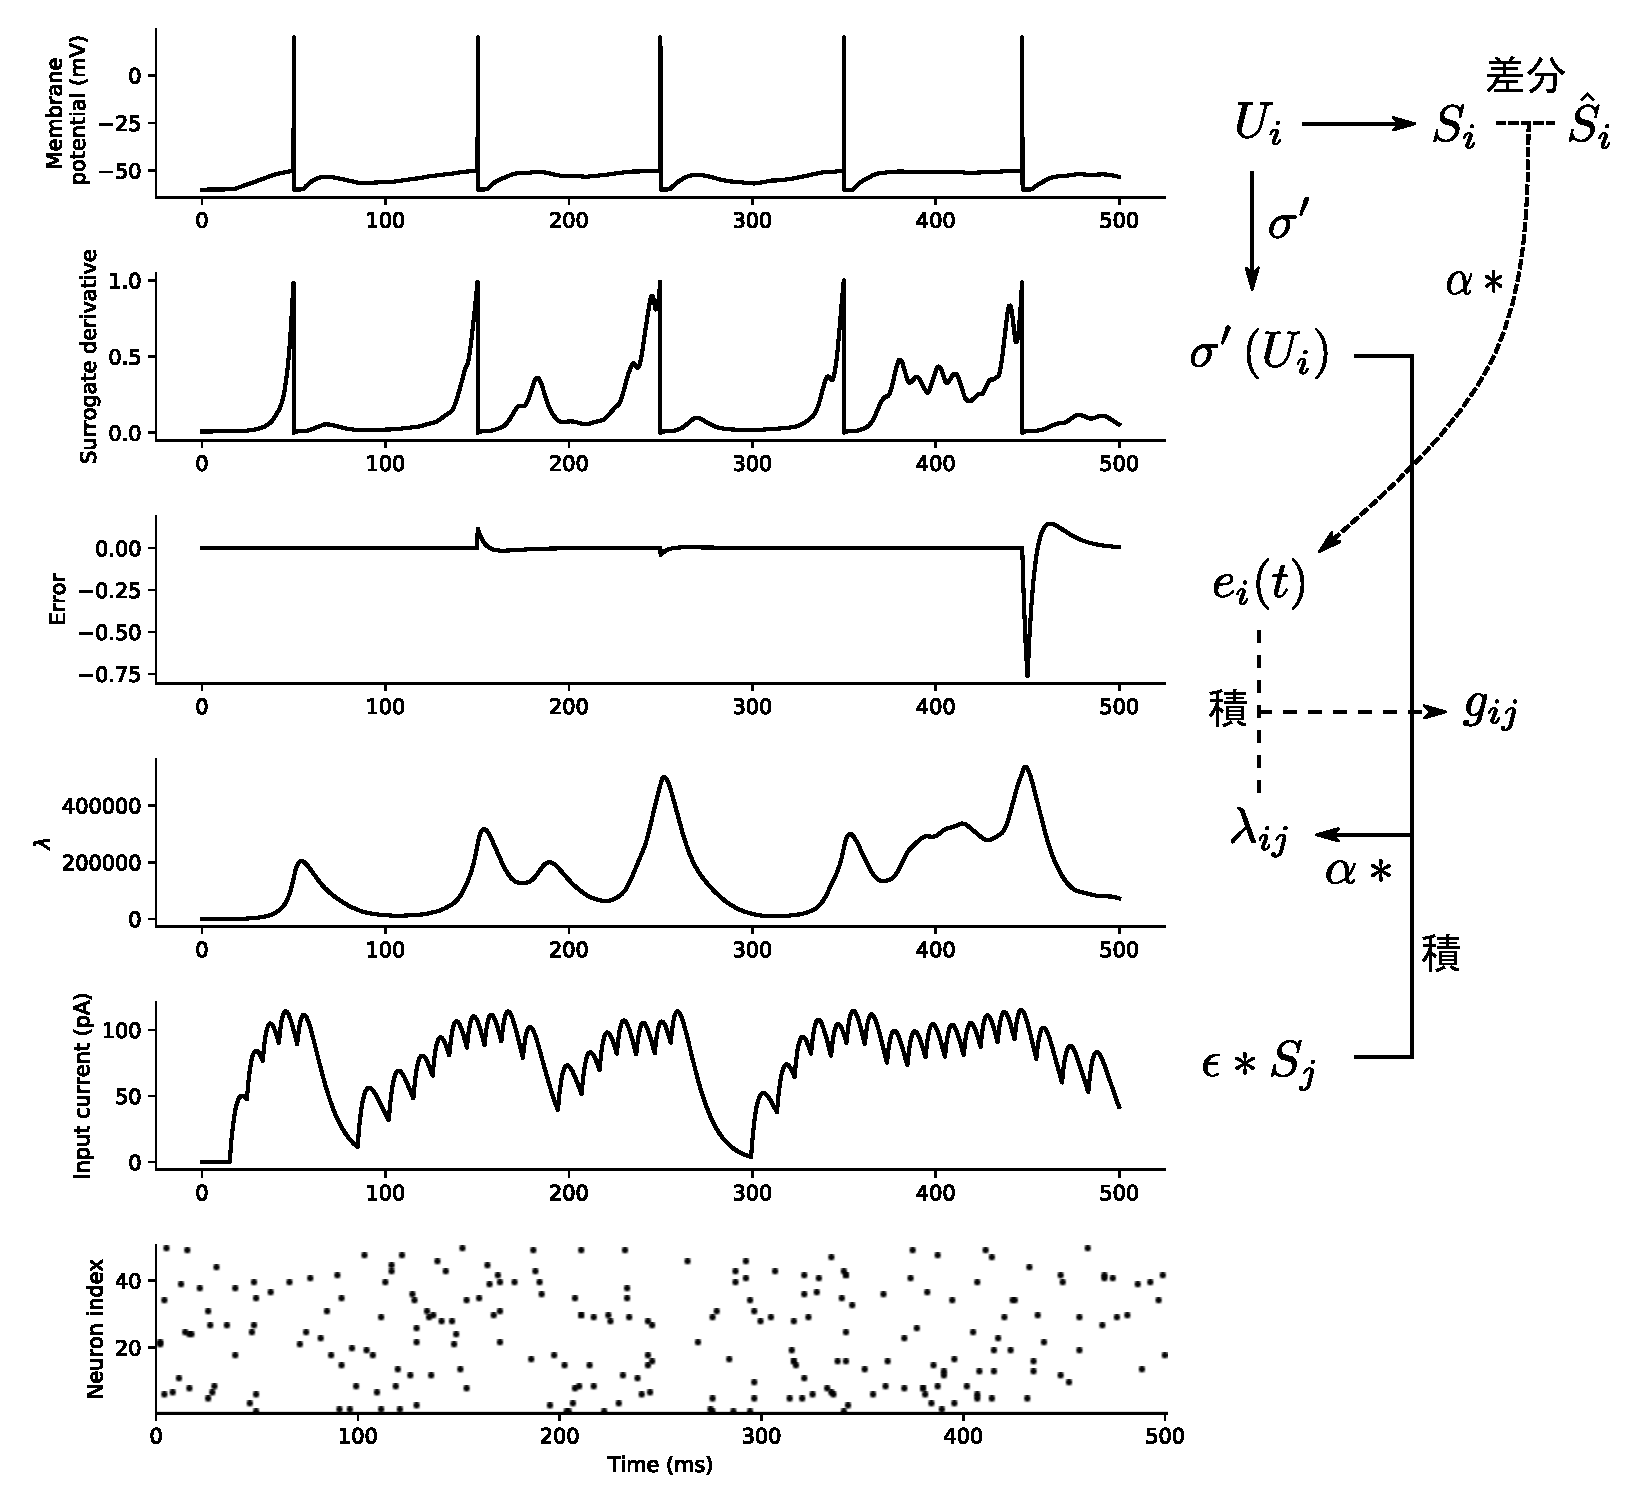
\includegraphics[scale=0.45]{figs/super_spike_2.pdf}
    \caption{SuperSpike法の結果とアルゴリズム。上から出力層の膜電位$U_i$, 高速シグモイドによる膜電位の微分の近似$\sigma^\prime (U_i)$, 出力層における誤差信号$e_i$, 適格度トレース$\lambda_{ij}$, 2層目の$j=0$番目のシナプス後電流$\epsilon * S_j$, 入力のポアソンスパイクを表します。}
    \label{fig:super_spike}
\end{figure}
\begin{figure}[htbp]
    \centering
    \includegraphics[scale=0.45]{figs/super_spike_cost.pdf}
    \caption{誤差関数の推移。(左)対称フィードバックの場合。(右)Feedback alignmentの場合}
    \label{fig:super_spike_2}
\end{figure}
